% Figure: worst per-job excess over FCFS, unguarded and under Guard(600),
% for the clean score and the three corrupted ones, at the three loads.
% Clean-score pair: the block headers of Table 5 of the manuscript (SPJF-E max excess
% 1,241.4 / 3,044.5 / 5,904.5 s) and its Guard(600) "Max exc." rows
% (492.2 / 507.8 / 523.7 s).  Corrupted pairs: Table~\ref{tab:s_adv}, columns
% "Max excess" unguarded / guarded.  Both tables come from
% outputs/paper_tables/.  No new computation.
\begin{figure}[htbp]
\centering
\resizebox{\textwidth}{!}{%
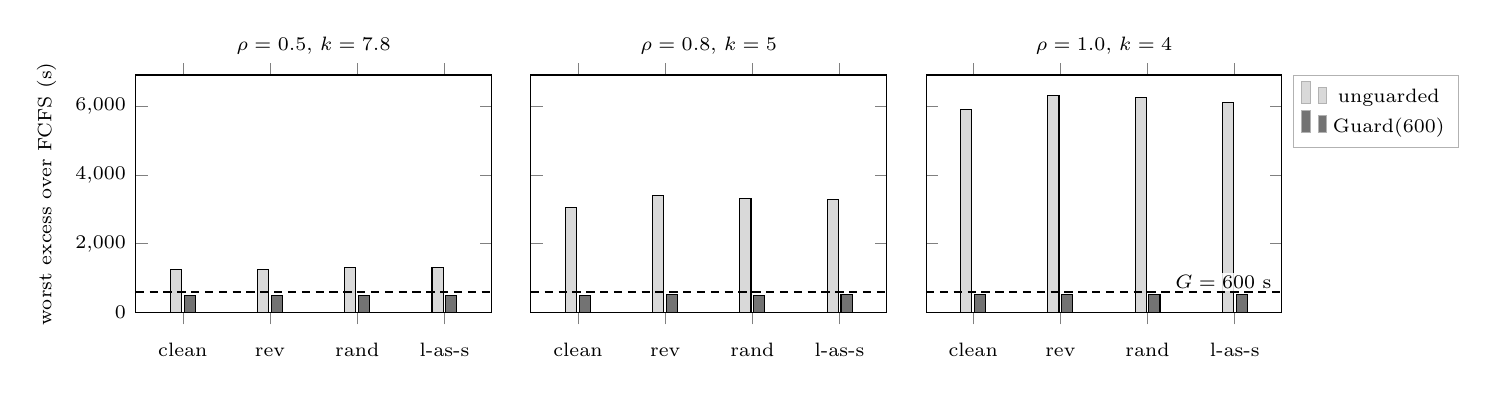
\begin{tikzpicture}[font=\footnotesize]
% RR-28: the x tick labels were rotated 40 degrees and cramped against each other in the
% narrow first panel, and the promise annotation sat at the left edge of that panel, where
% the y axis clipped it.  The panels are wider, the labels are set horizontally at
% \scriptsize (they are short enough), and the annotation moved into the third panel.
\pgfplotsset{
  excaxis/.style={
    width=6.1cm, height=4.6cm, ybar=1pt, bar width=4pt,
    symbolic x coords={clean,rev,rand,l-as-s}, xtick=data,
    ymin=0, ymax=6900, enlarge x limits=0.18,
    tick label style={font=\scriptsize}, label style={font=\scriptsize},
    title style={font=\scriptsize, yshift=-2pt},
    % text height/depth fixed so that the four labels share a baseline: with the default
    % anchor=north the box height follows the ascenders and "rev" would ride higher.
    x tick label style={anchor=north, yshift=-1pt, text height=1.6ex, text depth=0.45ex},
  },
}
\begin{axis}[excaxis, ylabel={worst excess over FCFS (s)},
             title={$\rho = 0.5$, $k = 7.8$}, name=q1]
  \addplot[fill=black!15] coordinates {(clean,1241.4) (rev,1240.1) (rand,1307.7) (l-as-s,1305.8)};
  \addplot[fill=black!55] coordinates {(clean,492.2) (rev,497.1) (rand,489.9) (l-as-s,497.1)};
  \draw[densely dashed] ({rel axis cs:0,0}|-{axis cs:clean,600}) -- ({rel axis cs:1,0}|-{axis cs:clean,600});
\end{axis}
\begin{axis}[excaxis, title={$\rho = 0.8$, $k = 5$}, yticklabels={},
             at={(q1.east)}, anchor=west, xshift=5mm, name=q2]
  \addplot[fill=black!15] coordinates {(clean,3044.5) (rev,3387.9) (rand,3319.4) (l-as-s,3292.0)};
  \addplot[fill=black!55] coordinates {(clean,507.8) (rev,513.5) (rand,504.5) (l-as-s,516.1)};
  \draw[densely dashed] ({rel axis cs:0,0}|-{axis cs:clean,600}) -- ({rel axis cs:1,0}|-{axis cs:clean,600});
\end{axis}
\begin{axis}[excaxis, title={$\rho = 1.0$, $k = 4$}, yticklabels={},
             at={(q2.east)}, anchor=west, xshift=5mm,
             legend style={font=\scriptsize, at={(1.03,1.0)}, anchor=north west,
                           draw=black!30, row sep=-1pt}]
  \addplot[fill=black!15] coordinates {(clean,5904.5) (rev,6295.7) (rand,6235.5) (l-as-s,6107.8)};
  \addlegendentry{unguarded}
  \addplot[fill=black!55] coordinates {(clean,523.7) (rev,534.8) (rand,520.7) (l-as-s,534.7)};
  \addlegendentry{Guard(600)}
  \draw[densely dashed] ({rel axis cs:0,0}|-{axis cs:clean,600}) -- ({rel axis cs:1,0}|-{axis cs:clean,600});
  \node[anchor=south east, font=\scriptsize, fill=white, fill opacity=0.85,
        text opacity=1, inner sep=1pt]
       at ({rel axis cs:0.98,0}|-{axis cs:clean,600}) {$G = 600$ s};
\end{axis}
\end{tikzpicture}}
\caption{Original-score reference and its corrupted-score controls. The worst single job, with and without the guard, under the
expected-cost score (``clean'') and the three corrupted scores of
Table~\ref{tab:s_adv}: reversed (rev), random (rand) and truly-longest-called-shortest
(l-as-s). The dashed line is the promise $G = \devnum{600}$ s. Sources: the clean
pair is the block header and the Guard($\devnum{600}$) row of
Table~4 of the manuscript; the three corrupted pairs are the ``Max excess'' columns
of Table~\ref{tab:s_adv}. The unguarded bar grows with load and with corruption;
the guarded bar does not, which is the content of Theorem~\ref*{M-thm:guard} of the manuscript and
not a property of the trace.}
\label{fig:excess}
\end{figure}
